\chapter{Software}

\section{Firmware}

Firmware finálního prototypu je určen především pro ovládání analogové části, vzorkování napěťového a proudového signálu a následný výpočet impedance. 
Je napsán pro mikrokontrolér STM32F103C8 v prostředí PlatformIO s frameworkem Arduino. 
Pro části, které se dotýkají časování a nastavení ADC, je však použita přímo knihovna STM32 HAL.

Program po spuštění inicializuje komunikační rozhraní, řídicí výstupy, zdroj měřicího signálu, indikační LED a snímací část. 
Poté  v hlavní smyčce pouze zpracovává příkazy ze sériové linky. 
Samotné měření tedy není spuštěno trvale, ale vždy až na požadavek z počítače.

\subsection{Komunikační rozhraní}

Zařízení je ovládáno textovým příkazovým rozhraním po sériové lince je k tomu využita knihovna SimpleCLI \cite{SimpleCLI}. 
Rozhraní slouží jak pro nastavování generátoru a analogového frontendu, tak pro vyvolání snímání nebo výpočtu impedance.

Mezi hlavní příkazy patří:
\begin{table}[H]
    \centering
    \small
    \begin{tabular}{ll}
        \toprule
        Příkaz & Význam \\
        \midrule
        \texttt{status} & Vypíše aktuální nastavení. \\
        \texttt{dds <frekvence> <povoleni>} & Nastaví frekvenci a zapnutí zdroje měřicího signálu. \\
        \texttt{amp <hodnota>} & Nastaví amplitudu měřicího signálu. \\
        \texttt{offset <hodnota>} & Nastaví stejnosměrnou složku signálu pomocí PWM. \\
        \texttt{range <hodnota>} & Vybere bočník pro změnu měřicího rozsahu. \\
        \texttt{vpga <hodnota>} & Nastaví zesílení napěťového kanálu. \\
        \texttt{ipga <hodnota>} & Nastaví zesílení proudového kanálu. \\
        \texttt{capture} & Sejme a odešle jeden z měřicích kanálů. \\
        \texttt{capturepair} & Sejme a odešle oba měřicí kanály. \\
        \texttt{measure} & Sejme oba kanály a vypočítá impedanci. \\
        \bottomrule
    \end{tabular}
    \caption{Přehled podporovaných příkazů firmwaru}
    \label{tab:firmware_prikazy}
\end{table}

Odpovědi jsou záměrně jednoduché a mají podobu řádků oddělených čárkou. 
To umožňuje snadné algoritmické zpracování na straně počítače a zároveň jednoduché ruční testování v sériovém terminálu.

\subsection{Řízení zdroje měřicího signálu a rozsahů}

Zdroj měřicího signálu je založen na obvodu . 
Mikrokontrolér ovládá obvod AD9837 sériovým rozhraním. 
Při změně frekvence firmware vypočítá ladicí slovo podle hodinového kmitočtu 16 MHz 
a zapíše jej do frekvenčního registru DDS. 
Výstup lze také softwarově zapnout a vypnout.

Amplituda výstupního signálu je nastavována digitálním potenciometrem MCP4561 přes sběrnici I\textsuperscript{2}C. 
Firmware zapisuje hodnotu 0 až 255 do jeho registru jezdce. 
Stejnosměrná složka zdroje je nastavována změnou střídy PWM výstupu, který je v analogové části filtrován.

Proudový rozsah a zesílení obou měřicích větví jsou řízeny jako tři dvoubitové hodnoty na šesti digitálních výstupech. 

\subsection{Synchronní snímání signálů}

Měřené střídavé signály jsou přivedeny na dva analogové vstupy mikrokontroléru. 
Protože pro výpočet impedance je důležitý nejen poměr amplitud, ale i fázový rozdíl,
musí být oba kanály vzorkovány současně.

Firmware k tomu využívá dvojici \acs{A/D} převodníků v režimu současné pravidelné konverze. 
Spouštění převodu zajišťuje časovač TIM3, jehož událost update je přivedena jako externí trigger pro ADC1. 
Po každém impulzu časovače tedy vznikne jeden synchronní pár vzorků.

Výsledky převodu jsou ukládány pomocí \acs{DMA} do paměťového bufferu. 
Každá položka bufferu je 32bitové slovo, ve kterém je v dolních 16 bitech uložen vzorek napěťového kanálu a v horních 16 bitech vzorek proudového kanálu. 
Maximální délka jedné dávky je 2048 dvojic vzorků.

Vzorkování je dávkové. 
Hostitelský počítač pošle požadovaný počet vzorků a požadovanou vzorkovací frekvenci. 
Firmware podle požadované frekvence nastaví děličku a periodu časovače TIM3, spustí ADC a DMA, 
počká na dokončení přenosu a po skončení časovač i převodníky zastaví. 
Protože časovač používá celočíselné dělení, skutečná frekvence nemusí být přesně rovna požadované hodnotě; 
firmware proto v odpovědi vždy vrací skutečně nastavenou hodnotu.

Pokud je požadovaná vzorkovací frekvence v příkazu zadána jako nula, 
firmware ji automaticky odvodí z aktuální frekvence DDS. 
Cílem je 25 vzorků na periodu měřicího signálu, při měřicí frekvenci větší než 40 kHz 
je však dosažen hardwarový limit vzorkovací frekvence 1 MHz a počet vzorků na periodu se snižuje.

Získané vzorky jsou následně buď odeslány po sériové lince do PC, nebo je z nich vypočítána impedance 
(v závislosti na použití příkazu \texttt{capture} nebo \texttt{measure}).

\subsection{Výpočet impedance}

\subsection{Stavová indikace}

Pro jednoduchou kontrolu běhu programu je použit výstup na signalizační LED. 
Firmware na něm generuje signál PWM s pomalu se měnící střídou a tím vizuálně indikuje, 
že hlavní smyčka běží a mikrokontrolér není zablokovaný.

Pro další signalizační účely jsou na DPS zapojené dvě adresovatelné RGB diody, 
ale v současnosti nejsou ve firmwaru nijak implementovány.

\section{PC aplikace}

K obsluze zařízení sice postačí textový terminál sériové linky, 
ale pro pohodlné používání a automatizované funkce je vhodné použít doprovodnou aplikaci \texttt{LCR\_meter\_app.py}.

Tato aplikace je napsaná v jazyce Python a poskytuje grafické uživatelské rozhraní.

\subsection{Základní měření}

\begin{figure}[H]
    \centering
    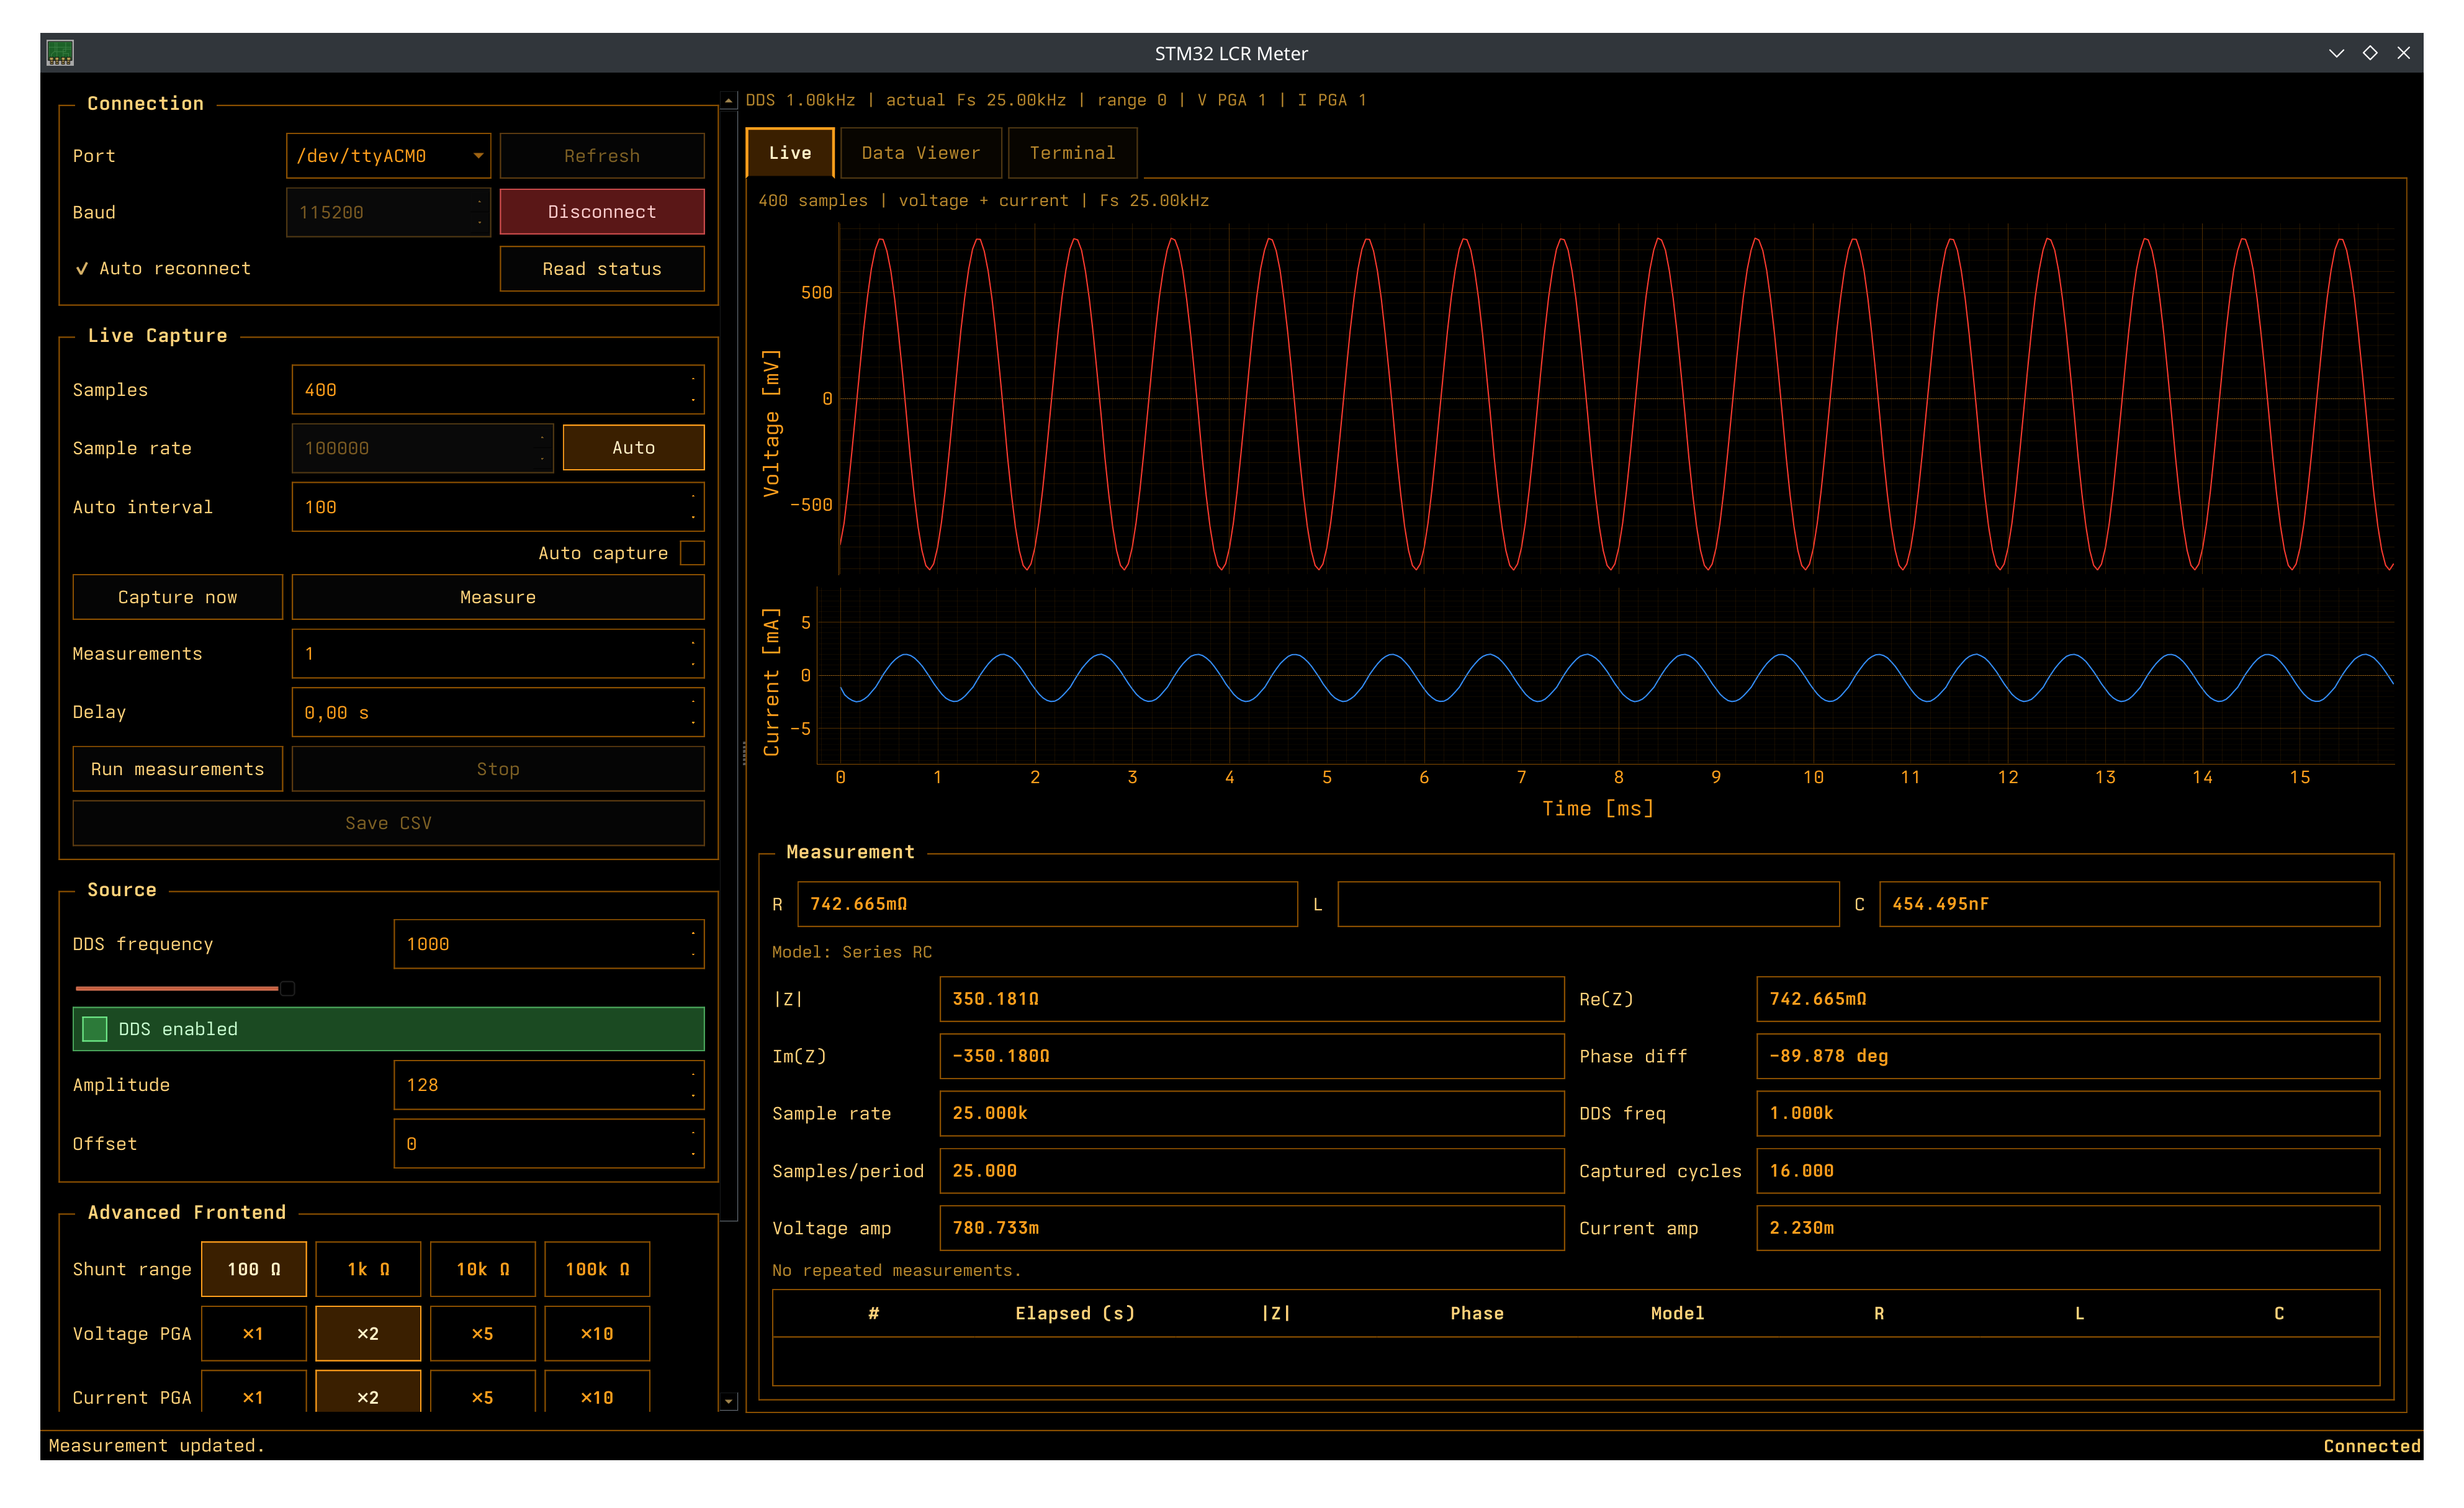
\includegraphics[width=\textwidth]{obrazky/basic_meas.png}
    \caption{Hlavní okno aplikace při základním měření}
    \label{fig:pc_app_basic_meas}
\end{figure}

V levé části aplikace jsou ovládací prvky přístroje, lze zde nastavit všechny parametry a odesílat příkazy měření.

Tlačítkem Capture now lze požádat o navzorkování napětí a proudu.
Tyto vzorky se náledně v pravé části zobrazí v osciloskopickém grafu.
Při aktivaci Auto capture je požadavek o vzorky odesílán periodicky, grafy se v čase aktualizují.

Jelikož v přístroji není implementována žádná funkce automatického nastavení rozsahu, je toto zobrazení
užitečné pro ruční nastavení. Čím větší je amplituda zobrazených grafů, tím přesněji přístroj měří.
Zároveň je vhodné na grafech zkontrolovat, zda není přítomné výrazné rušení nebo zda nejsou signály ořezané rozsahem ADC.

Tlačítko Measure také vede k navzorkování napětí a proudu, 
v tomto případě se do PC neposílají samotné vzorky ale již vypočítaná impedance.

Výsledky se zobrazí v pravé dolní části. Aplikace z impedance také odvodí hodnoty RC nebo RL. Výpočet probíhá podle vzorců:

\begin{equation}
    Z = R + jX
\end{equation}

\begin{equation}
    L = \frac{X}{2\pi f}, \quad \text{pro } X > 0
\end{equation}

\begin{equation}
    C = -\frac{1}{2\pi f X}, \quad \text{pro } X < 0
\end{equation}

\subsection{Statistické zobrazení}

Dále tato aplikace umožňuje automatizované mnohonásobné měření a následné statistické zpracování.
Tato funkce se spouští tlačítkem Run measurements po zadání množství měření a případného časového rozestupu mezi nimi.

Po dokončení měření se pravá část přepne na záložku Data Viewer, 
kde se zobrazí histogram a jemu přizpůsobená gaussova křivka.
Numerické statistické hodnoty jsou pak zobrazeny vlevo od grafu.

Naměřená data lze také uložit do souboru CSV, který pak lze v záložce Data Viewer opět otevřít.

\begin{figure}[H]
    \centering
    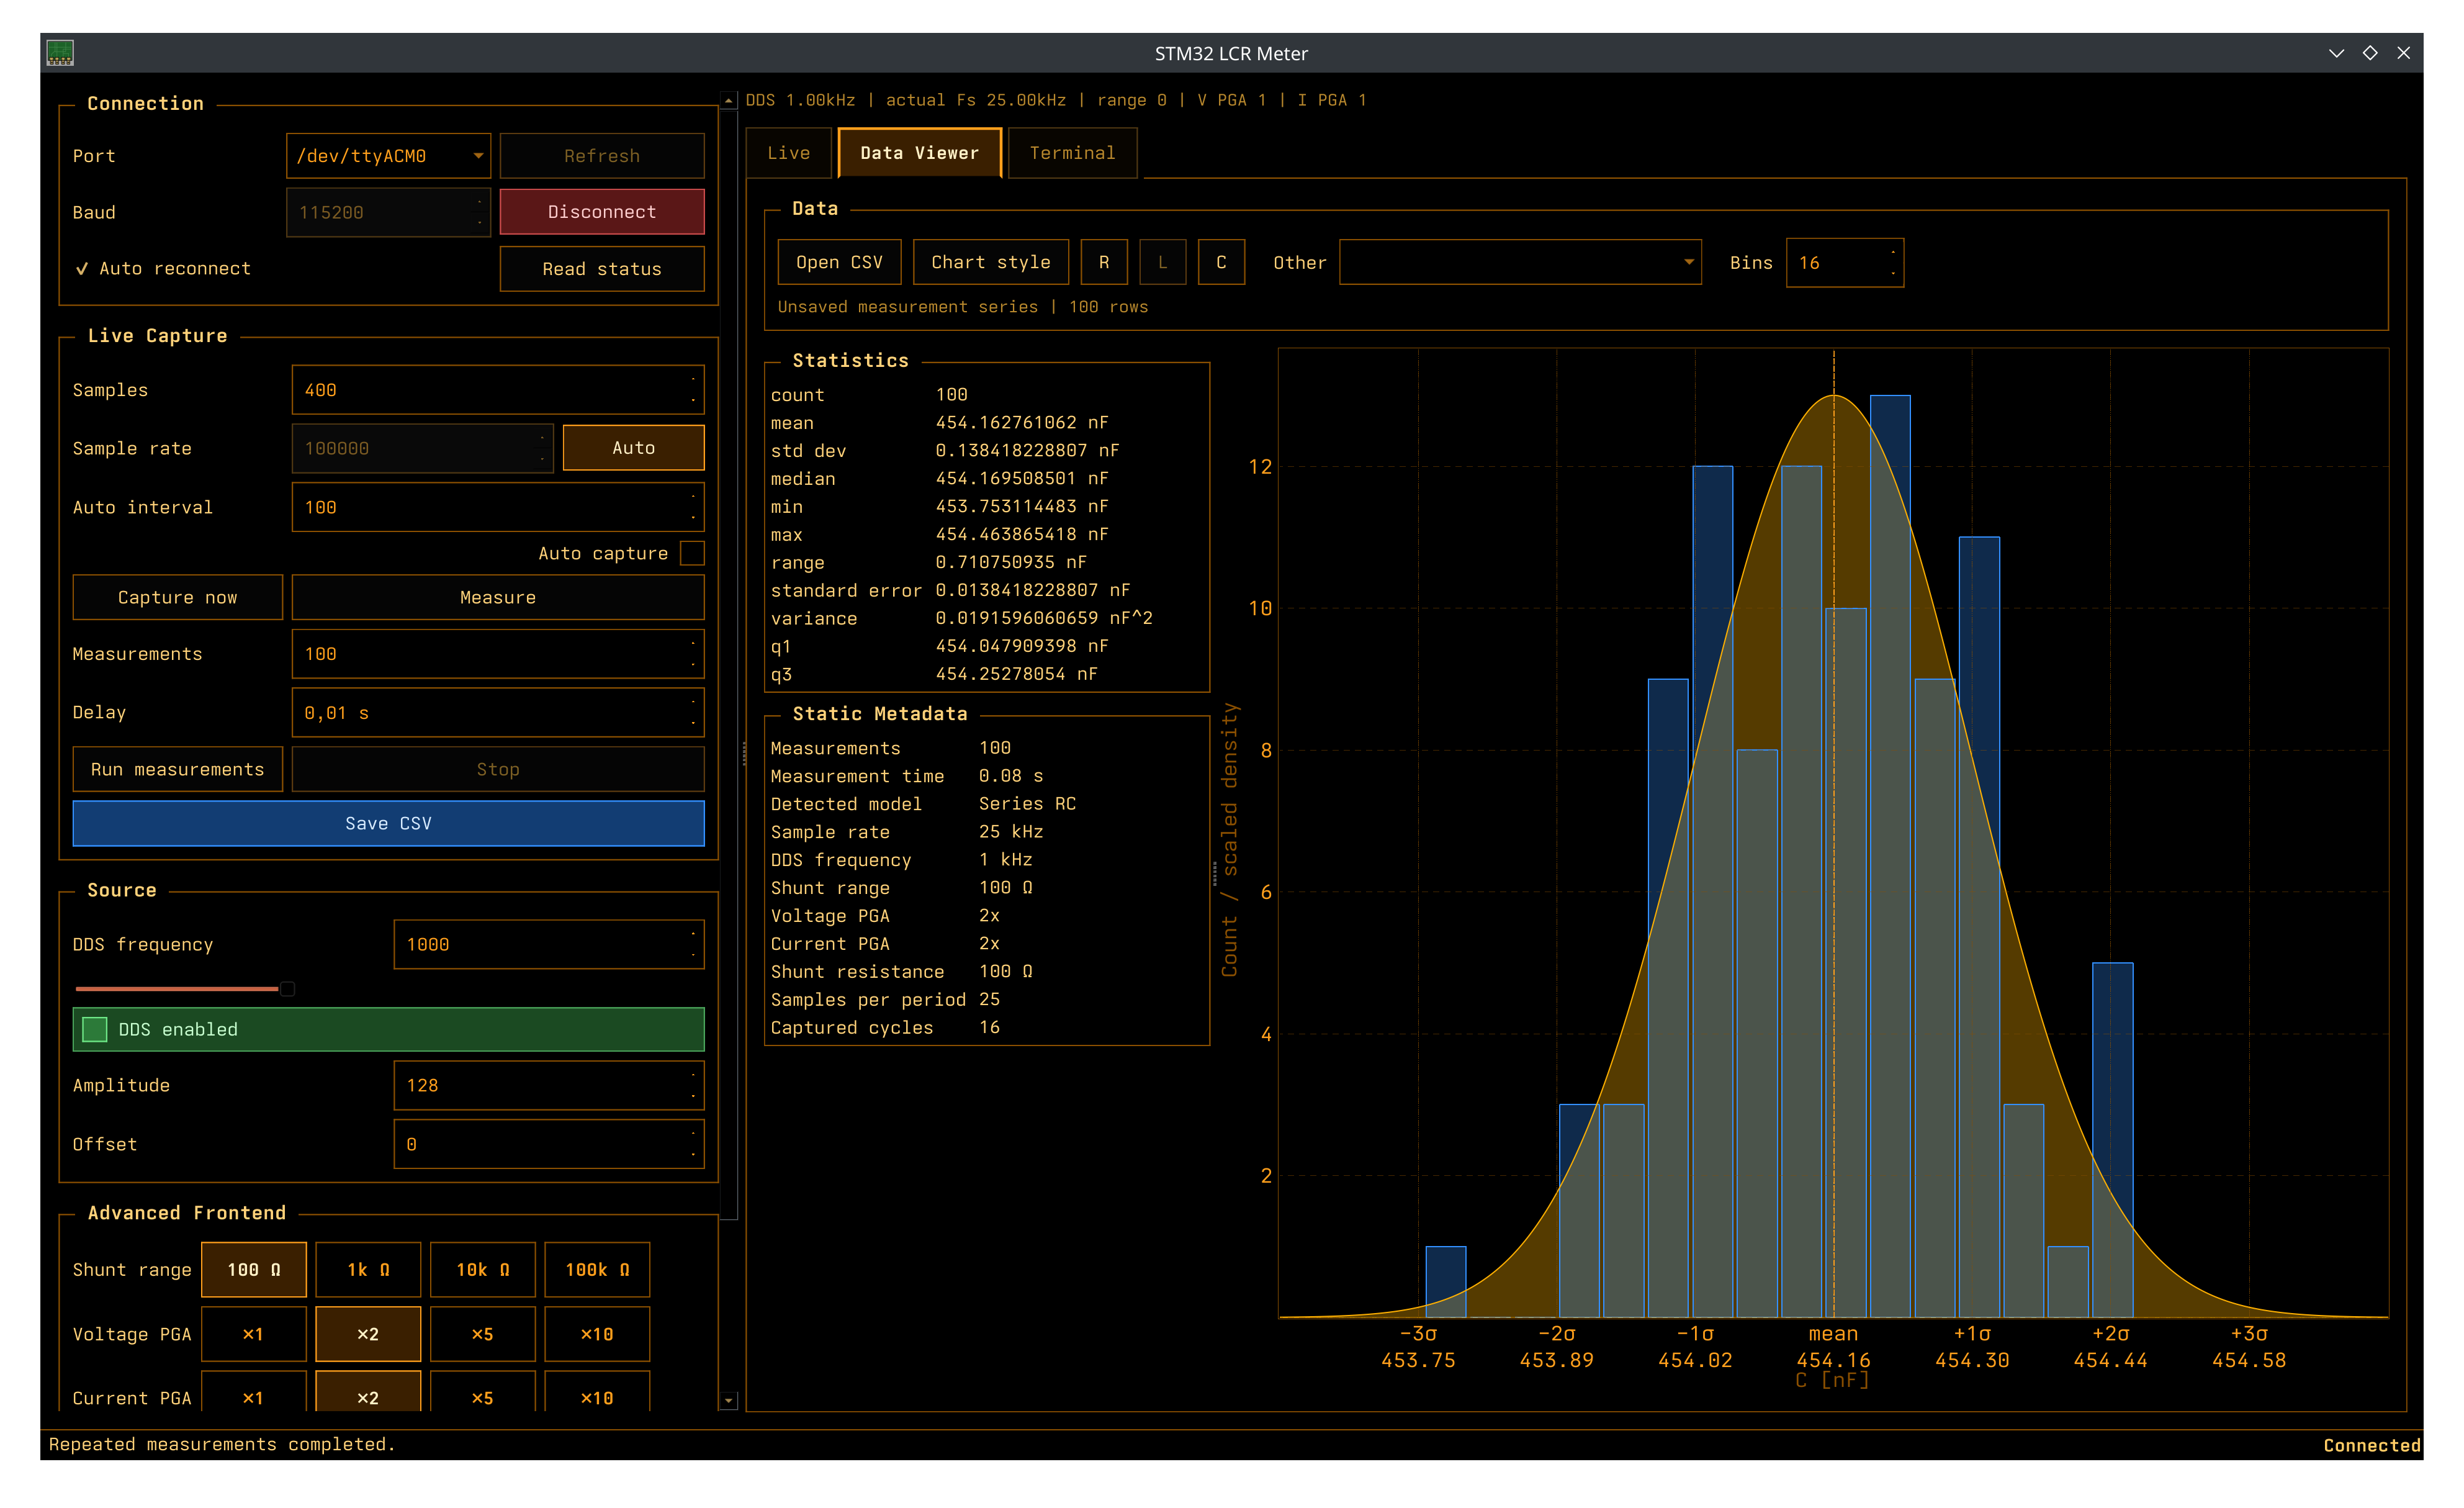
\includegraphics[width=\textwidth]{obrazky/stats_meas.png}
    \caption{Statistické zobrazení opakovaných měření v aplikaci}
    \label{fig:pc_app_stats_meas}
\end{figure}

\subsection{Integrovaný terminál}
Doplňkovou funkcí aplikace je záložka Terminal, 
která umožňuje nahlédnout na komunikaci se zařízením po sériové lince
a případňe ručně zadat příkaz. Při běžném použití to však není potřebné.

\begin{figure}[H]
    \centering
    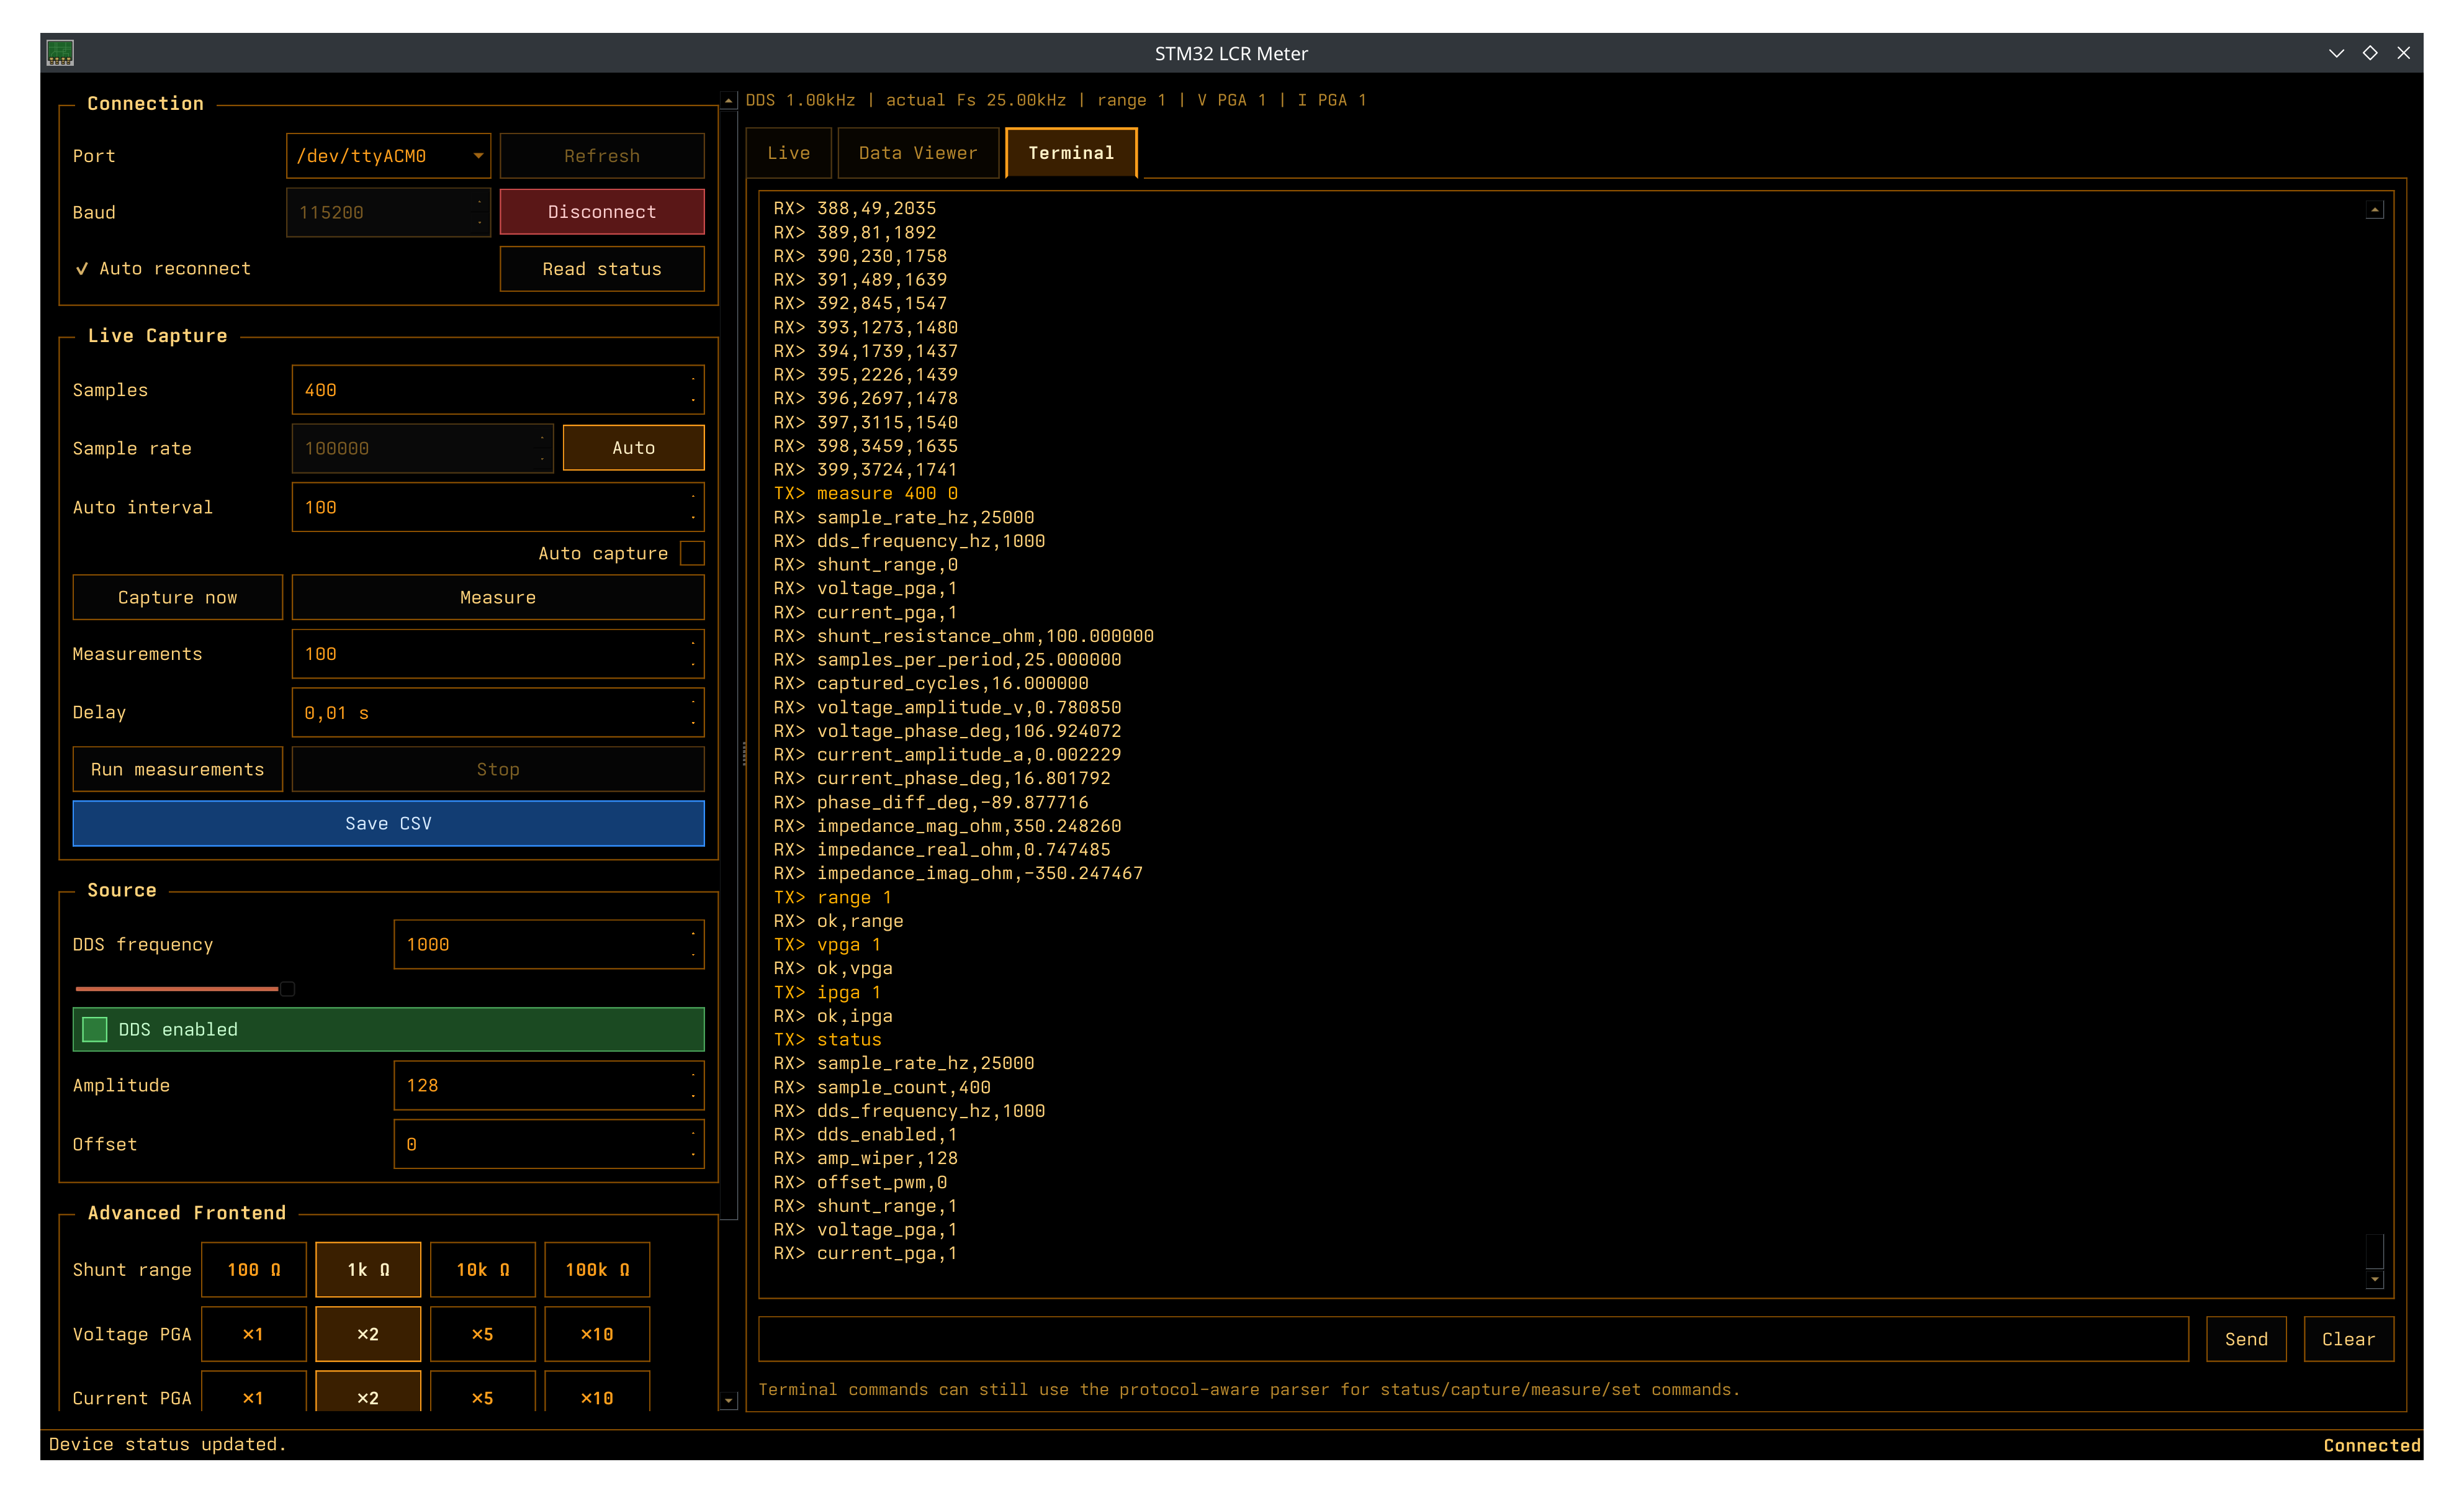
\includegraphics[width=\textwidth]{obrazky/integrovany_terminal.png}
    \caption{Integrovaný terminál aplikace pro ruční zadávání příkazů}
    \label{fig:pc_app_terminal}
\end{figure}
